\chapter{Exploratory Data Analysis}
\label{cha:Data analysis}
In this chapter details of the dataset are introduced and an analysis is performed. Things discussed about the dataset concern assessing missing data, removing zero days, normalizing the data and removing time-series with identified fundamental changes The analysis looks at the seasonality,  influence of temperature, comparing weekdays with weekends, impact of holidays and the driving households characteristics. Finally the definition of a suitable baseline model is given, which will be used during the evaluation with more elaborate models in chapter \ref{cha:Evaluating results}.

% Look at the comments during the meeting 'writing the WTK thesis'.
% Make sure that write every part sufficient substantiated.

\section{Data description}\label{s:Data description}
% how the dataset is made up --> use the information of the competition.
\textbf{update pictures}
The data that is used in this thesis is made available for the \href{https://ieee-dataport.org/competitions/ieee-cis-technical-challenge-energy-prediction-smart-meter-data}{IEEE-CIS technical challenge on energy prediction from smart data}. It consists out of data from smart meters about the 1/2 hour granulated electricity consumption of $3248$ households located in the United Kingdom in the year $2017$. The definition of a household are all the people who occupy a single housing unit, regardless of their relationship to one another. Each smart meter collected thus a total of $17520$ measurements that are performed by the the leading international energy provider, E.ON UK plc. Not all the $3248$ smart meters consist of full data as can be seen in Figure \ref{fig:amountNaN} in appendix \ref{app:A}. It can be clearly seen that there are $12$ steps in the amount of missing values. This is because the available data ranges from one month (only December) to a full year of data. This acknowledges that customers may have joined at different times during the year. Additionally, missing values are introduced due to errors in sending/receiving from smart meters.\\
Next to the electricity consumption of the different households, also information is available about the average, minimum and maximum temperature of the day on the location of the smart meter. This data is available at a daily resolution. Also, through voluntary surveys, incomplete information is collected about $2143$ smart meters. This concerns e.g. dwelling type, number of occupants, number of bedrooms etc. Table \ref{tab:attributes} displays all the attributes in appendix \ref{app:A}.\\

%After substituting the missing values as discussed in \ref{s:missing_data}, all the available weeks are averaged out over all the $270$ smart meters that contain a full year of measurements. The result is given by Figure \ref{fig:averaged_week}. A difference that with belgian load profiles is the consumption peak after midnight. This is due to the higher use of the electric storage heaters used in the UK. These systems store electric energy when the electric tariff is low e.g. overnight and releases the heat when the tariff is high.

\begin{table}
	\footnotesize
	\hspace{1cm}
	\begin{tabular}[t]{@{}ll}\hline
		\textbf{consumption.csv}&\\ \hline
		\# households &3248 \\ 
		information & electric load\\
		measurements & 17520\\
		granularity&$ \frac{1}{2} $hour\\ 
		timespan&year 2017 \\    
		location&UK\\ \bottomrule   
	\end{tabular}
	\hspace{2cm}
	\begin{tabular}[t]{@{}ll}\hline
		\textbf{weather.csv}&\\ \hline
		information & average temperature\\
		& max temperature\\
		& min temperature\\
		granularity& daily\\ \hline \hline
		\textbf{addInfo.csv}&\\ \hline
		\# households &2143 \\ \bottomrule		    
	\end{tabular}
	\hfill
	\caption{Table with information about the characteristics of the available datasets.}
	\label{tab:available_data}
\end{table}

Because of the additional information about the attributes that are summed up in Table \ref{tab:attributes}, it can be better understood what kind of households are included in the consumption.csv. It is assumed that all the loads are measured form households of the type listed below and each household is made up of maximum four persons and has a maximum of five bedrooms. industrial loads or small businesses, a bakery for example, are not considered.

\begin{itemize}
	\item flat
	\item bungalow
	\item detached house
	\item semi-detached house
	\item terraced house
\end{itemize}


\section{Preprocessing}\label{s:Preprocessing}

Following steps discuss the preprocessing done on the consumption time-series containing measurements for the entire year. 

\subsection{Missing data} \label{s:missing_data}
\textbf{It should be made clear that this section about missing values is only applied during the data analysis.}
As discussed above the consumption dataset contains additionally to the missing months also missing data due to sending/receiving errors of the smart meters. When this happens the data of the whole day is lost. It should be emphasized that a missing value should not always directly be seen as an error. It can be that the smart meter was put off because the inhabitants were on a holiday for example. The nan values then also gives information about the consumption behaviour, namely that it is possible that the inhabitants go on vacation and the electrical load will in this case normally correspond to a constant base load. However, the assumption is made that in the case of the ``consumption.csv'' missing data corresponds to a sending/receiving error of the smart meter. This assumption is valid because when full year data is assessed, the missing values always perfectly correspond to a day of missing values. It is therefore highly likely that the organizers of the competition manually deleted days in the consumption to increase the difficulty of the forecasting and to model sending/receiving errors of the smart meters. That the missing values correspond to sending/receiving errors is also stated in the data description of the competition.\\

 Two methods to impute the missing values are compared. Method one substitutes the missing values of a time-serie by the mean of all the measurements done by the meter. Method two replaces the missing values by the mean consumption value of the same moment on the next and previous day. If the next or previous day is also missing, the closest known day is used. The resulting signals can be seen in Figure \ref{fig:mv_mean} and Figure \ref{fig:mv_s} in appendix \ref{app:A}.\\
 

In order to ascertain which method of the two performs the best, a reference dataset is needed in order to compare the estimated with the true values of the missing measurements. From the original dataset which contain $ 3248 $ meters it was found that for $ 181 $ meters the month March was given without missing data. These $ 181 $ complete signals of the month March are used as reference dataset. In order to create the test data in each of the $ 181  $ meter signals $ 7 $ random days of the month March were removed and estimated by the earlier two methods. The normalized mean square errors, $ MSE_{AN} $ and $ MSE_{mean} $ given by $ \sum_{i=1}^{D} e_i^2  $ and normalized by $ MSE_{mean} $ are given in Figure \ref{fig:mv_result}.

\begin{figure}[h!]
	\centering
	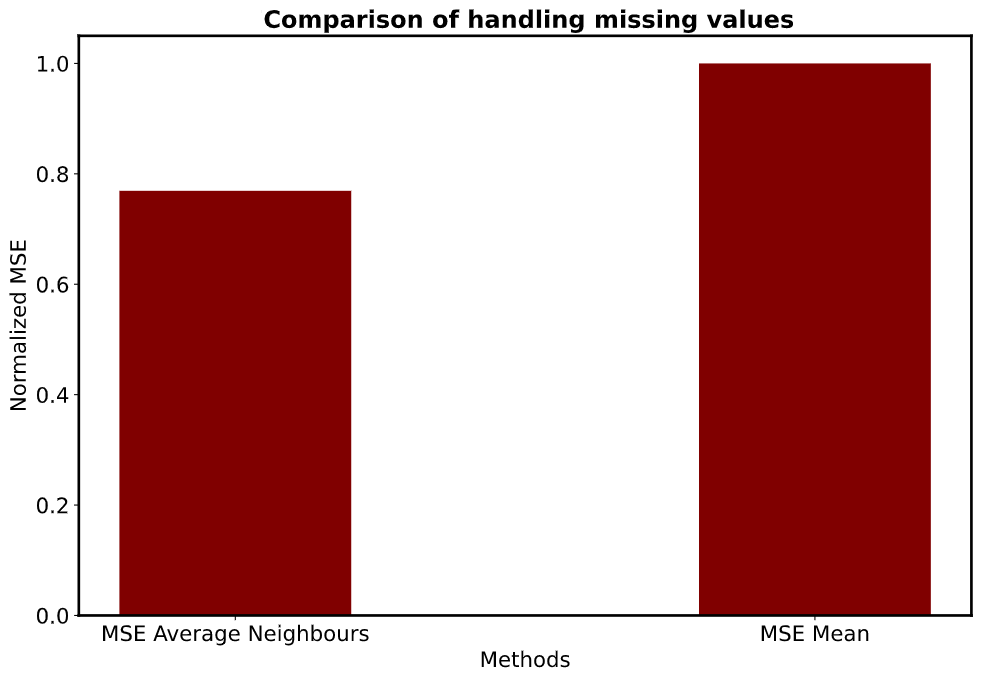
\includegraphics[width=0.8\textwidth]{mv_result.png}
	\caption{Resulting month of March after substitution of the missing values by the mean value of the measurements. }
	\label{fig:mv_result}
\end{figure}

From Figure \ref{fig:mv_result} it can be seen that using method $ 2 $ which estimates the missing values by the mean consumption value of the same moment on the next and previous day, outperforms method $ 1 $ which takes the mean of the signal. Therefore, all the missing values in the consumption dataset are estimated using method $ 2 $ with the only exception the first of January and thirty-one December. If one of these two days are missing, the method $ 1 $ is used because of the absence of two neighbouring days. 

%%%%%%%%%%%%%%%%%%%%%%%%%%%%%%%%%%%%

\subsection{Zero days}

When processing the consumption data, some untraditional meter measurements were identified. For example there were $ 9 $ meters that had multiple days with zero day consumption measurements. Because it is unlikely that a household produces exactly zero kWh on a day all these $ 9 $ meters were removed. The consumption time-serie of one of the meters is displayed in Figure \ref{fig:zero_con} in appendix \ref{app:A}.\\

\begin{figure}[h!]
	\centering
	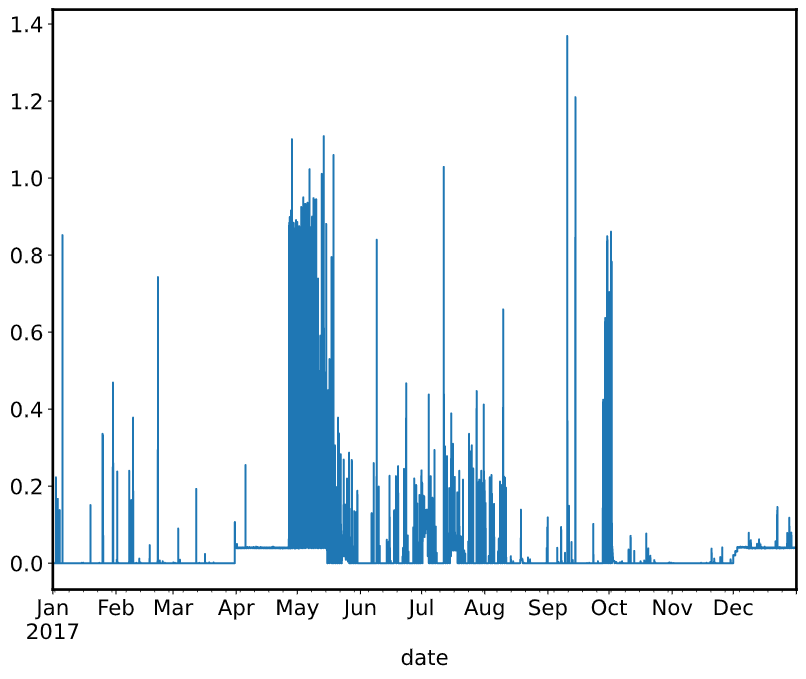
\includegraphics[width=0.6\textwidth]{zero_con.png}
	\vspace*{-5pt}
	\caption{One of the $9$ identified meters with multiple zero daily consumptions}
	\label{fig:zero_con}
\end{figure}


%%%%%%%%%%%%%%%%%%%%%%%%%%%%%%%%%%%%


Also, there has been looked if there were fundamental changes in the electricity consumption of certain meters. This is further discussed in section \ref{s:Removing of fundamental changes in the consumption load}.


\subsection{Normalization of the data}
\label{s:Normalization of the data}
\textbf{it should be made clear that this normalization is only here used.}
% normalize as done in ppt --> deviding by the yearly consumption.
% downside of this normalilzation that outshooters will have influence.
Normalization is necessary because while absolute consumption differs, relative patterns of human behaviour are more similar \cite{Lago2020}. The patterns in the human behaviour is what a forecasting model is trying to predict and normalization contributes by avoiding the disturbance of different magnitudes in which this human pattern may occur. Every individual household time-serie is normalized based on its yearly consumption as was done in \cite{Lago2020}. The advantage of using the yearly consumption to normalize in comparison of the minimum and maximum values, is the robustness against measurements out shooters and every smart meter has a total consumption of one at the end of the year

\begin{equation}\label{eq:norm}
	normalized\hspace{0.3cm} value = \frac{consumption_i}{\sum_{n=1}^{17520} consumption_i}.
\end{equation} 

As discussed in section \ref{s:Data Analysis} the average is taken over all the normalized time-series to obtain a single signal.  


\subsection{Removing of fundamental changes in the consumption load} 
% want to do assumption that there is no fundamental change in training data.
After normalization of all the individual time-series it is looked for fundamental changes in the consumption load due for example when an extra person lives in the house or when systems are installed that use a lot of electricity during the year. An example of such a time-serie can be seen in Figure \ref{fig:fundamental_change} in appendix \ref{app:A}.
These changes are identified by looking at the maximum difference of the minimum and maximum rolling mean consumption over $ 7 $ days for each individual meter. If this difference can not anymore be explained by the dependency on the temperature and previous present appliances, it is assumed that a fundamental change in electricity consumption took place. 
%It is desired that the mean consumption doesn't change much during the year. This is because the model that later will be used expects the household situation to be the same for the entire year and the time-series with a fundamental change can thus lead to a disturbance when it is kept in the training data.
 Figure \ref{fig:fund_change} shows all the maximum differences between the minimum and maximum weekly rolling averages. The red line on shows the cutoff and the smart meters above this line are defined as outliers and removed. The definition of an outlier that is used is the one and a half times the interquartile range. In total $ 256 $ smart meters remain. 

%In Figure \ref{fig:f_c} in appendix \ref{app:A} the time-serie with the new maximum difference between the minimum and maximum weekly rolling averages is given.

\begin{figure}[h!]
	\centering
	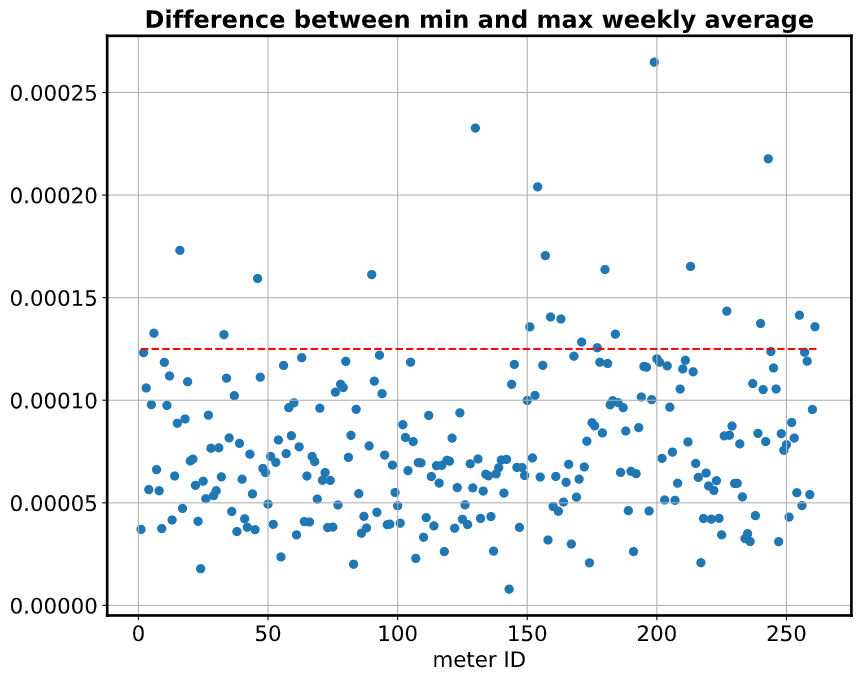
\includegraphics[width=0.8\textwidth]{fund_change.png}
	\caption{The maximum differences between the minimum and maximum weekly rolling averages for all the different time-series.}
	\label{fig:fund_change}
\end{figure}



%\cite{NarjesFallah2018}

\section{Data Analysis}\label{s:Data Analysis}
% Aggregation of the different signals is necessary in order to be able to make predictions.
Finally, the average is taken over all the remaining $256$ time-series to obtain a single signal. This is done to investigate the dependency of the smart meters on seasonality, temperature, weekends and holidays. At the end of this chapter a baseline forecasting will be discussed that will be used as null-hypothesis in chapter \ref{cha:Evaluating results} to assess if the developed models lead to an improvement.

% An individual household consumption time-serie is much subdued to complex and personal decisions that cause increases or decreases of the consumption. It is hard to capture all theses effects in a single model. By aggregation of the individual time-series by taking the average, this noisy individual behaviour is mitigated. The aggregated signal is now modelled and the increase or decrease of the consumption can be explained by a small set of variables. The aggregated signal can be seen as a ``virtual distribution substation'' as discussed in \cite{Hoverstad2015}. 
 


\subsection{Seasonality}
In this section the seasonality of the consumption data is discussed. In \cite{Hoverstad2015}it was concluded that all the forecasting algorithms that were considered, produced more accurate forecasts when they were combined with a preprocessing stage that extracted the seasonality before forecasting, compared to applying the same algorithms directly on raw data. The forecasting model is left with the task of modelling the deviation from the template consumption instead of performing a forecast out of the blue. However in \cite{Hoverstad2015} they made forecasts of an aggregated signal which has a reasonably amount of regularity which is not the case for electrical consumption of individual households. These templates or filters are extracted from the consumption dataset by the use of equations \ref{eq:daily_filter} and \ref{eq:weekly_filter}. $ D $ and $ W $ gives respectively the number of days and weeks in the dataset. $\bar{y}_i$ and $\bar{y}_j$ gives the consumption of half an hour, averaged over respectively all days and weeks. 

\begin{equation}\label{eq:daily_filter}
	\bar{y}_i = \frac{1}{D} \sum_{d=1}^D y_{di}, \hspace{10mm} i \in [1,48],
\end{equation} 

\begin{equation}\label{eq:weekly_filter}
	\bar{y}_j = \frac{1}{W} \sum_{w=1}^W y_{wj}, \hspace{10mm}  j \in [1,336].
\end{equation} 



Figure \ref{fig:daily_filter} shows the daily filter in appendix \ref{app:A}. Figure \ref{fig:weekly_filter} shows the weekly filter.

\begin{figure}[h!]
	\centering
	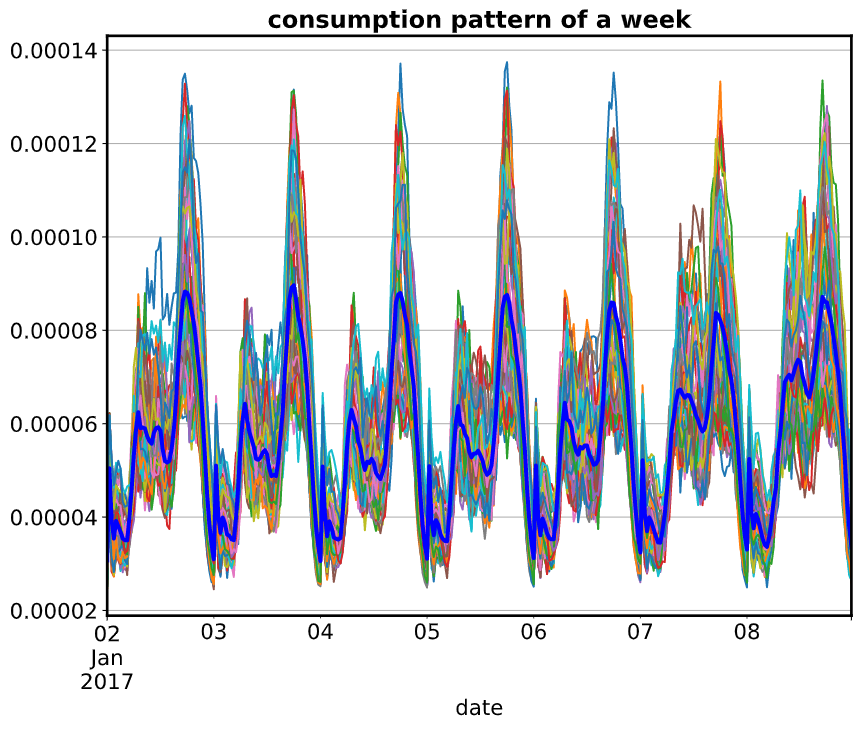
\includegraphics[width=0.8\textwidth]{weekly_filter.png}
	\caption{The seasonality of the electrical load during the week. The blue line shows the average week over all weeks in $ 2017 $. }
	\label{fig:weekly_filter}
\end{figure}

% plot the moving average of the year. Clearly see the impact of the summer and winter.
% This is a trend that can be taken into account when predicting.


In the daily and weekly filters there can clearly be seen a consumption peek after midnight. This is due to heat storage systems that use electricity in the hours of low tariff and that release heat during high electricity tariffs. 

\subsection{Comparing weekdays with weekends} \label{s:Comparing weekdays with weekends}
Weekdays vs weekends can be compared with the help of Figure \ref{fig:weekly_filter}. The reader is reminded that in order to get this graph, all the remaining household loads after preprocessing are averaged after which all the weeks are again averaged using equation \ref{eq:weekly_filter}. It can be seen that the consumption of the average business day is similar to a weekend day concerning the two main peaks during the day (7 am and 6 pm) and the sharp peak at midnight. However, it can be seen that the first peak during the day is higher and goes less down again during the weekend. This effect can be seen both during a Sunday and Saterday, but is most visible during a sunday. To proof previous statements similarity is measured by calculating the hourly difference of the $ 21 $ combinations that can be made of two different days. Figure \ref{fig:similarity_weekday} shows in blue and orange the error of combinations between business days or weekend days and in green the error of combinations between a business day and weekend day. The error value is calculated by summing the hourly errors between two days. It can be clearly seen that when a business day and weekend day are combined the error (green) is bigger and thus similarity smaller. Another thing that can be noticed is that the left cluster of green dots corresponds to a Saterday and the right to a Sunday. It can be noticed that Saterdays are more similar to a business day than a Sunday. 

\begin{figure}[h!]
	\centering
	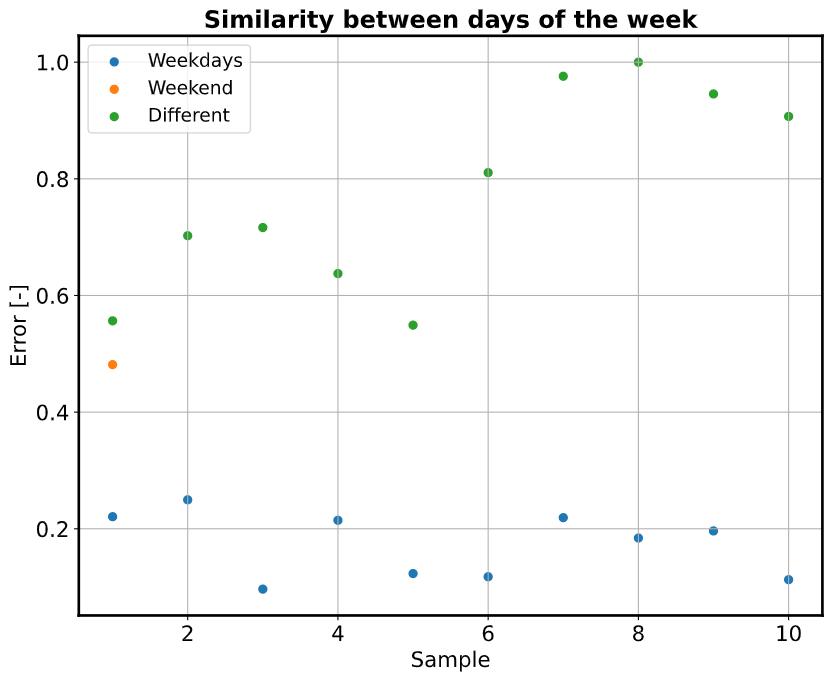
\includegraphics[width=0.8\textwidth]{similarity_weekdays.png}
	\caption{Error between different pairs of weekdays.}
	\label{fig:similarity_weekdays}
\end{figure}


\textbf{Add here more specific how the error is calculated between holiday and weekday --> MAE and normalized.}

\subsection{Impact of holidays}\label{s:Impact of holidays}
% important that look at holidays in the UK. In paper \cite{Hoverstad2015} all the holydays are subsitued by the same day the next week and the previous week. It is possible to look at all the holidays, normalize them concerning temperature and try to get a seasonality model. 
In order to look at the impact of a holiday, all the holidays of the English and welsh holiday calendar are identified for the year $ 2017 $. For each of the $ 8 $ holidays a corresponding business day is selected with an as close as possible average temperature of the day. This is done to mitigate the temperature dependency. The resulting average holiday and business day is given in Figure \ref{fig:bvsh}. A holiday behaves similar to a weekend day with the first peak load going higher and goes less down over time. Figure \ref{fig:sim_weekdays} shows that a holiday behaves the most similar to a Sunday .

It can be seen that the consumption of a holiday behaves similar as a weekend day. Figure shows the average error between a holiday vs business day and a holiday vs weekend day. The error is calculated as discussed in section \ref{s:Comparing weekdays with weekends}. 

\begin{figure}[h!]
	\centering
	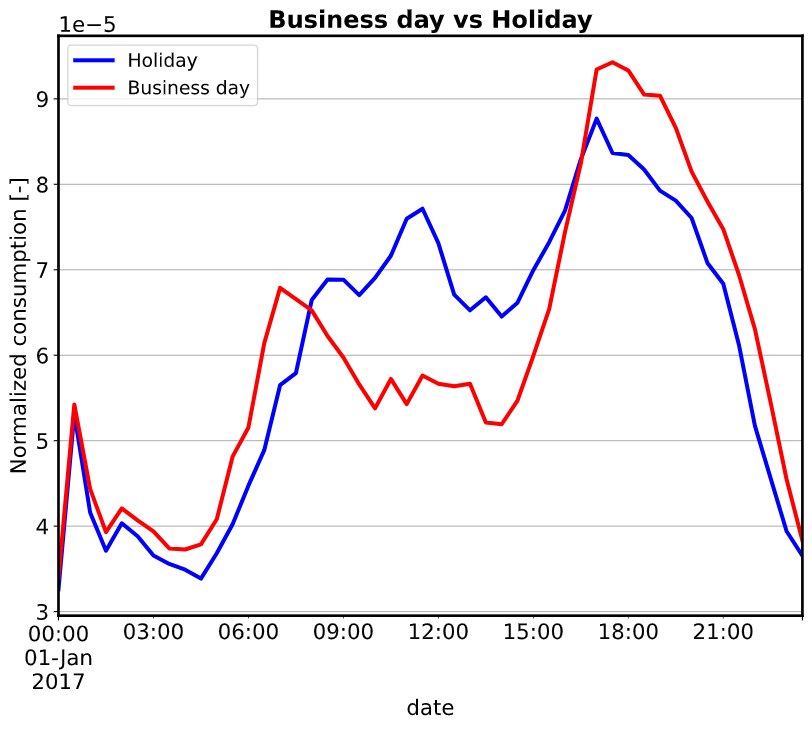
\includegraphics[width=0.8\textwidth]{bvsh.png}
	\caption{Figure with the comparison between holidays and business days.}
	\label{fig:bvsh}
\end{figure}

\begin{figure}[h!]
	\centering
	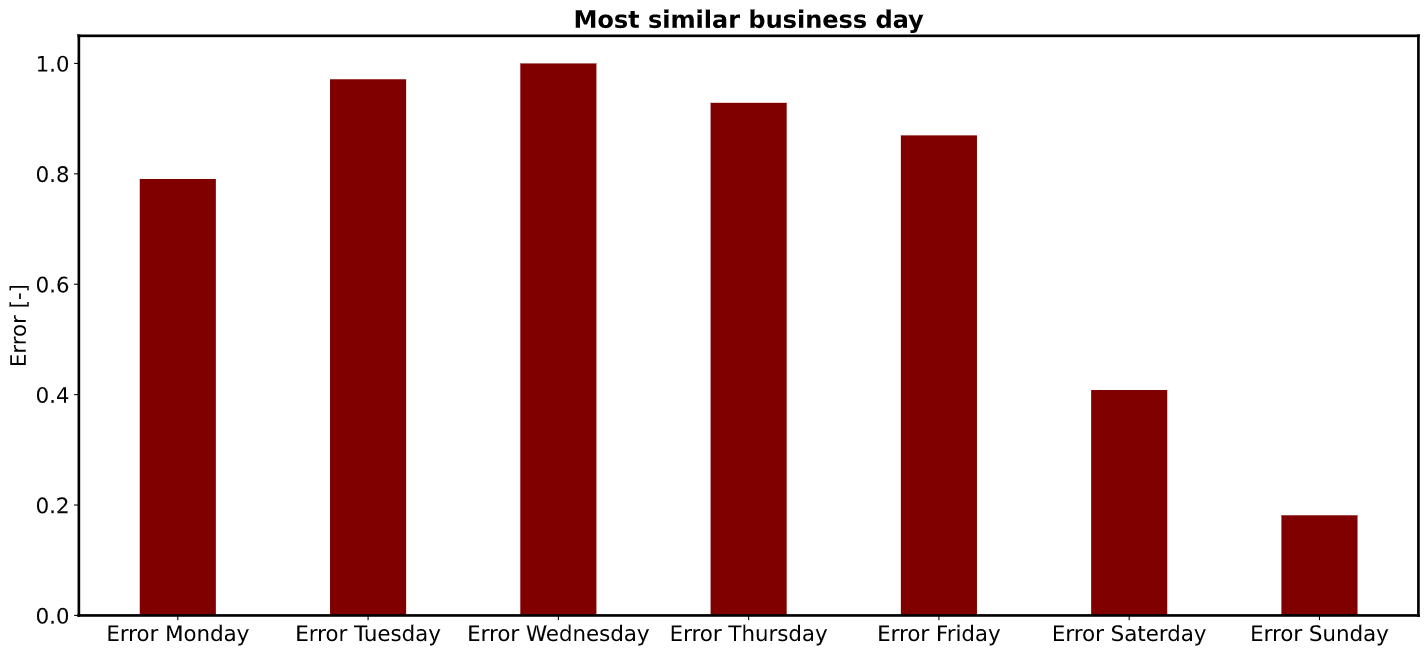
\includegraphics[width=1.0\textwidth]{sim_weekdays.png}
	\caption{Error between a holiday and other days of the week.}
	\label{fig:sim_weekdays}
\end{figure}


\subsection{Influence of temperature}
% notes on correlation see OneNote.
% use the correlations. https://realpython.com/numpy-scipy-pandas-correlation-python/
% resample the consumption to daily and then apply some of the correlation techniques. 
In following section the correlation between the temperature and the electricity consumption is discussed.\\


\textbf{Pearson correlation}\\
The Pearson correlation is a measurement of the linear dependency between two variables which is based on the covariance variable. A Pearson correlation value gives information concerning the magnitude of the association and the corresponding direction of it. A Pearson value of one and minus one give respectively a perfect positive and negative linear relation between the variables. A value of zero, corresponds to independent behaviour. Following formula is used when calculating the Pearson correlation

\begin{equation}\label{eq:pearson}
	\rho_{X,Y} = \frac{\sigma_{x,y}}{\sigma_x\sigma_y}.
\end{equation}

Assumptions concerning Pearson correlation are that samples used for the correlation should be independent drawn, come in pairs, follow homoscedasticity and there are no outliers. Outliers are especially undesirable when there are not a lot of samples. The variables should be normal distributed, linear related to each other and be continuous.\\
The samples used for the correlation are generated by calculating the daily consumptions matched with the daily average temperature. In this case the above assumptions are thus not valid. Homoscedasticity is important when performing linear regression and assumes that $ \sigma_x $ and $ \sigma_y $ are constant. This assumption is validated by making use of Figure \ref{fig:pearson}.

\begin{figure}[h!]
	\centering
	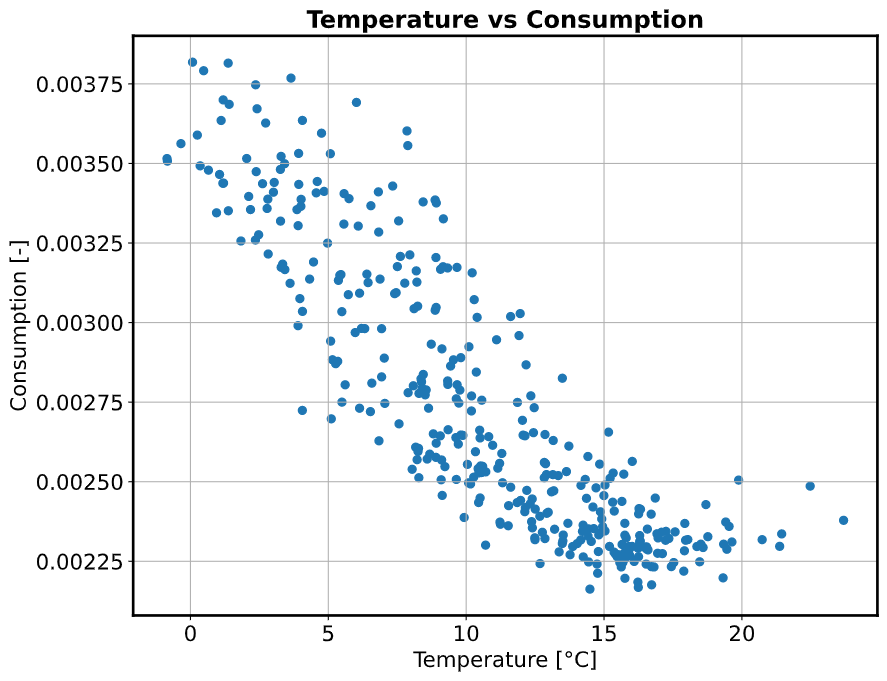
\includegraphics[width=0.8\textwidth]{pearson.png}
	\caption{Relation between normalized daily consumption and daily temperature.}
	\label{fig:pearson}
\end{figure}

This figure shows the classic cone-shaped pattern of heteroscedasticity. On days when it is warm there is overall similar human behaviour in lowering the electricity consumption. However, on colder days the variation in consumption is higher, which means that homoscedasticity is not fulfilled. Because the assumptions of the Pearson correlation are not fulfilled, care should be taken with its output.\\

Applying the Pearson correlation on Figure \ref{fig:pearson} gives a correlation value of $ -0.87 $. This means there is a reasonable linearly decreasing relation.\\


\textbf{Spearman correlation}\\
Spearman correlation is a ``Rank correlation''. This means that the ordering of the consumption and temperature in a sample are each compared in their corresponding array of measurements.  When the ordering of both variables in a sample are similar, correlation is strong and positive. If the ordering is reversed, correlation is strong and negative. There is a perfect positive ordering if larger consumption always corresponds to a higher temperature. Notice that for a perfect ordering, no linear relation of the variables is necessary. The Spearman correlation coefficient is calculated using equation \ref{eq:pearson}, but takes into account the rank of a variable in all the measurements of this variable instead of the measurement value itself.\\

In order to use the spearman correlation data has to be ordinal, which means that it can be ordered. The spearman correlation gives information about the monotonicity relation between the variables. $ \rho = 1 $ corresponds to a monotonically increasing relation.\\

Applying the Spearman correlation  gives a correlation value of $ -0.89$, which means there is a good negative monotone relation. This means if the temperature is higher, consumption is likely to be lower. Identically, if the temperature is lower it is likely that the consumption will be higher. \\

\textbf{Kendal correlation}
The ``Kendal correlation'' is also a rank based correlation. Here it is looked at the pairs of observation that are concordant, discordant or neither. A correlation coefficient close to one occurs when both variables have the same ranking and similar a coefficient close to minus one occurs when rankings in one variable are the reverse of the other. Equation \ref{eq:kendall} gives the equation to calculate the ``Kendal correlation coefficient''.

\begin{equation}\label{eq:kendall}
	\tau = \frac{n^+-n^-}{\sqrt{(n^++n^-+n^x)(n^++n^-+n^y)}}
\end{equation}
\begin{itemize}
	\item $ n^+ $ is the number of concordant pairs
	\item $ n^- $ is the number of discordant pairs
	\item $ n^x $ is the number of ties only in x
	\item $ n^y $ is the number of ties only in y
	\item concordant $\rightarrow $ $ (x_i > x_j ) $ and $ (y_i > y_j ) $ or $ (x_i < x_j ) $ and $ (y_i < y_j ) $
	\item discordant $\rightarrow $ $ (x_i > x_j ) $ and $ (y_i < y_j ) $ or $ (x_i < x_j ) $ and $ (y_i > y_j ) $
	\item neither $\rightarrow $ $ (x_i = x_j ) $ or $ (y_i = y_j ) $
	\item if both $ (x_i = x_j ) $ and $ (y_i = y_j ) $ $\rightarrow $ not included in either $ n^x $ or $ n^y $
\end{itemize}

Applying the Kendal correlation  gives a correlation value of $ -0.67$, which means there is a reasonable negative monotonicity relation.\\

% There is a clear dependency between temperature and electricity consumption, which means that electricity is used for heating.  



\subsection{Identification of driving attributes} \label{s:Identification of driving attributes}
In this section the influence of the extra knowledge about the kind of household where the smart meter is located, is investigated. This is not done by using a single averaged signal as was the case in the previous analysis sections. Now, every meter with additional information is considered. In Figure \ref{fig:bp_dwellingtype} the monthly consumption of the month December in function of dwelling type is shown. The month December is chosen, because this month is known for every smart meter. Missing values of the smart meters are substituted by method two, as discussed in section \ref{s:missing_data}. The amount of meters used for every visualization can be seen in Table \ref{tab:attributes}.

% Boxplots and consumptions are plotted. 

\begin{figure}[h!]
	\centering
	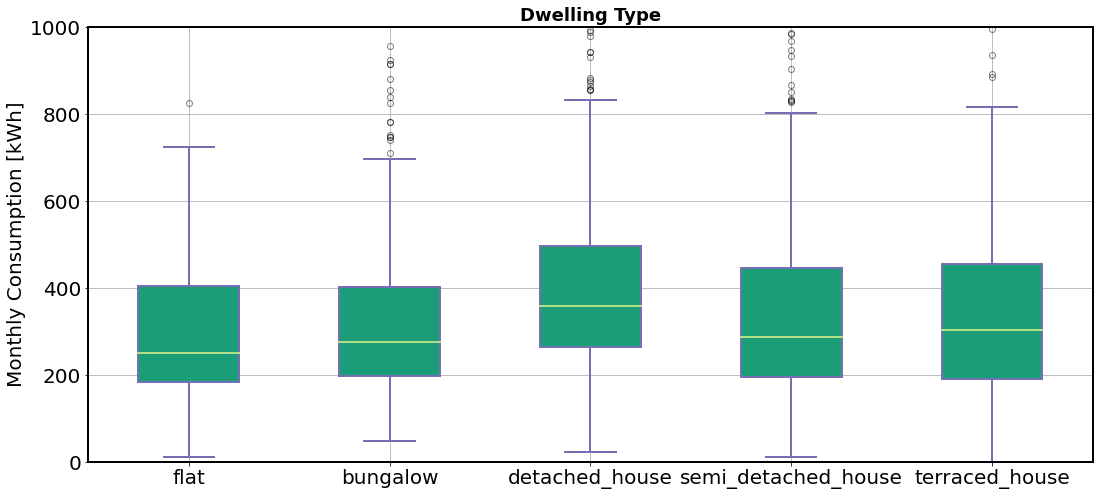
\includegraphics[width=1\textwidth]{bp_dwellingtype.png}
	\caption{Figure with the comparison of the different dwelling types.}
	\label{fig:bp_dwellingtype}
\end{figure}





Similar as was done in Figure \ref{fig:bp_dwellingtype} is also done for the other characteristics of the smart meters. The conclusions are listed below. As can be seen in Table \ref{tab:attributes}, some characteristics have not much data or the data is not much distribute over the different options of a characteristic. If this is the case, no reliable conclusions could be drawn. \textbf{Add concrete numbers!!}

\begin{itemize}
	\item There is a lot of variance in the monthly consumption of a detached house, but it has mostly a higher consumption than other dwelling types
	\item A ``real'' house (detached, semi-detached or terraced) tends to have higher monthly consumptions than a flat or bungalow.  
	\item The order of monthly consumption according to the mean and median values: Flat < Bungalow < Semi-detached < Terraced < Detached
	\item More occupants means more monthly consumption
	\item More rooms in the house means more monthly consumption
	\item Almost all houses use gas as heating fuel
	\item Almost all houses use gas as hot water fuel
	\item The age of the boiler has no clear effect on the monthly consumption
	\item The vast majority of the lofts are insulated
	\item The majority of walls are insulated
	\item The vast majority heats till a temperature between $ 18 $ and $ 20  $ degrees
	\item The majority of people has an efficient lighting percentage between $ 75\% $ and $ 100\% $
	
\end{itemize}



\section{Conclusion}
\textbf{Write a conclusion}
The final section of the chapter gives an overview of the important results
of this chapter. This implies that the introductory chapter and the
concluding chapter don't need a conclusion.




%Please don't abuse enumerations: short enumerations shouldn't use
%``\verb|itemize|'' or ``\texttt{enumerate}'' environments.
%So \emph{never write}: 
%\begin{quote}
%	The Eiffel tower has three floors:
%	\begin{itemize}
%		\item the first one;
%		\item the second one;
%		\item the third one.
%	\end{itemize}
%\end{quote}
%But write:
%\begin{quote}
%	The Eiffel tower has three floors: the first one, the second one, and the
%	third one.
%\end{quote}

%%% Local Variables: 
%%% mode: latex
%%% TeX-master: "thesis"
%%% End: 
